\documentclass[10pt,twocolumn,letterpaper]{article}

\usepackage{cvpr}
\usepackage{times}
\usepackage{epsfig}
\usepackage{graphicx}
\usepackage{amsmath}
\usepackage{amssymb}

% Include other packages here, before hyperref.

% If you comment hyperref and then uncomment it, you should delete
% egpaper.aux before re-running latex.  (Or just hit 'q' on the first latex
% run, let it finish, and you should be clear).
%\usepackage[pagebackref=true,breaklinks=true,letterpaper=true,colorlinks,bookmarks=false]{hyperref}

\cvprfinalcopy % *** Uncomment this line for the final submission

\def\cvprPaperID{****} % *** Enter the CVPR Paper ID here
\def\httilde{\mbox{\tt\raisebox{-.5ex}{\symbol{126}}}}

% Pages are numbered in submission mode, and unnumbered in camera-ready
\ifcvprfinal\pagestyle{empty}\fi
\begin{document}

%%%%%%%%% TITLE
\title{Scene Text Recognition in the Wild}

\author{Chen-Yu Lee and Phuc Nguyen\\
University of California, San Diego\\
{\tt\small chl260@ucsd.edu}
% For a paper whose authors are all at the same institution,
% omit the following lines up until the closing ``}''.
% Additional authors and addresses can be added with ``\and'',
% just like the second author.
% To save space, use either the email address or home page, not both
%\and
%Second Author\\Institution2\\First line of institution2 address\\
%{\tt\small secondauthor@i2.org}
}

\maketitle
\thispagestyle{empty}

%%%%%%%%% ABSTRACT
\begin{abstract}
This paper demonstrates an algorithm to tackle the problem of reading text in uncontrolled ``natural'' photos. In contrast to the traditional OCR problem, for which the focus was on scanned pages, scene text presents a number of challenges more commonly associated with general object recognition, including different viewpoints, sizes/scale, locations, fronts, and styles (neon, graffiti). There are two main contributions of this work: The first is the novel character detector using more representative information in the training step and support vector machine based classifier. The second is a more general word recognition system by setting up the dual of a Quadratic Programming problem. We show a significant improvement in accuracy on Street View Text dataset by 10% without explicit guide from lexicon.
\end{abstract}

%%%%%%%%% BODY TEXT
\section{Introduction}

For most people, a visual display of information is the fastest and most direct way to receive external information, through activities such as billboards and neon signs. However, for the visually impaired, it cannot be conveyed via the visual way to obtain information. In this paper, scene text recognition technique can be used in natural environments, so that the visually impaired person can access to the environmental information in texts.

Scene text recognition could also help improve map services. House number and store name recognition helps improve address geocoding. In most countries, very few addresses have associated geographic coordinates. The geocodes of the majority of addresses is therefore usually computed by interpolating the geocodes of neighboring addresses. Such interpolation introduces errors which may be significant, and may result in poor user experience. With the vehicle's location, the house number and the store name, a better map service of the building of interest can be computed in a straightforward way.

\begin{figure}[t]
\begin{center}
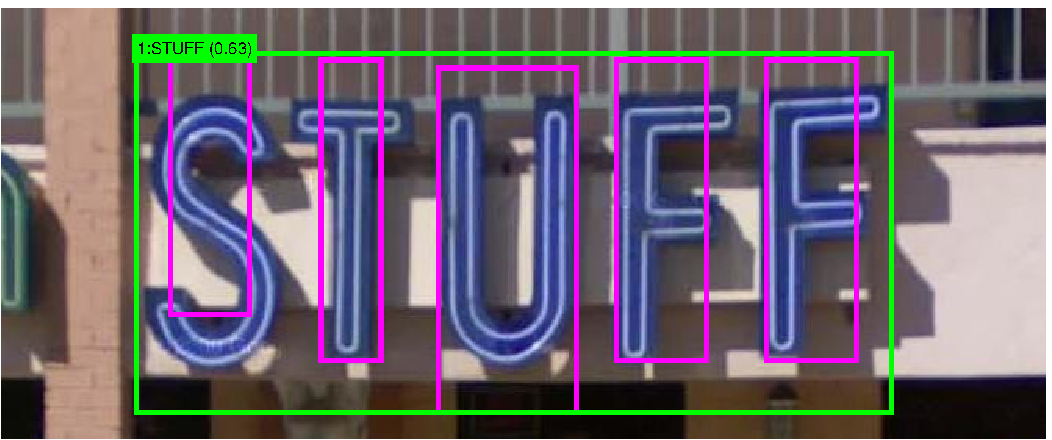
\includegraphics[width=1\linewidth]{fig/p1}
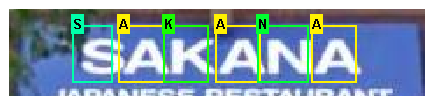
\includegraphics[width=1\linewidth]{fig/p10}
\end{center}
   \caption{Examples of character detection and word recognition.}
\label{fig:sample1}
\end{figure}

Smith and Learned-Miller~\cite{118} showe that the similarity among characters could be used to improve scene text recognition. They use bottom-up design by starting with hand segmentations of each character in the form of a rectangular bounding box, then the similarity expert performs on all pairs of bounding boxes within one word to higher the confident score of boxes that are the same in both signal and label spaces. This approach required highly rectified candidate bounding boxes (segmented by hand in~\cite{118}) to obtain reliable similarity output.

Neumann and Matas~\cite{120,119} use tradition pipelines for text recognition that their system first performs text localization by sequential selection from the set of Extremal Regions(ERs), and then use character segmentation approach to produce input for traditional Optical Character Recognition (OCR) engine. While this algorithm rely on stability of both text localization and segmentation procedure.

Netzer et al.,~\cite{121} detect and read house numbers from street level photos using unsupervised feature learning method. They show a robust feature learning approach that does not need to use any existing image descriptors and achieve high accuracy on their benchmark. The experiment setting is similar to our goal while they conduct text recognition on total $10$ classes (from $0$ to $9$) and need training dataset that contains around $73,000$ digits.

Mishra et al.,~\cite{111} propose a Conditional Random Field model to perform word recognition from candidate bounding boxes of each character obtained in similar method as our work. They impose top-down cues obtained from a lexicon-based prior and the optimal word representation is obtained by minimizing the energy function corresponding to the random field model.

While progress has been made on cropped word recognition recently, the main challenge still lies on ene-to-end word recognition on the full image due to a great amount of unpredictable false positive objects. Our work and experiment setting are based on~\cite{417} that we propose a more robust and reliable character detector to achieve a better scene text recognition on both cropped word and whole word recognition on full image.

%-------------------------------------------------------------------------
\section{Character Detection}

Each step of character detection will be discussed in detail.

\subsection{Character Detection with SVM}

Like many object recognition approaches, the first step in our algorithm is to detect potential locations of characters in the input image. In order to detect characters in different fonts and view points, we perform multi-scale and multi-aspect ratio for each character via sliding window classification. However, there are 62 categories (26 lowercase, 26 uppercase, and 10 digits) in our problem, we need to choose a suitable classifier in order to handle this large amount of categories efficiently. Multi-class Support Vector Machine (SVM)~\cite{122} is an robust classifier to deal with multi-class problem. In our implementation, we use Histogram of Gradient (HOG) descriptor~\cite{115}.

This sliding window detection method produces many possible locations with different scales and aspect ratios. We call them candidate bounding boxes. However, some of those candidate boxes are not useful for recognizing words in the next step. We eliminate those bounding boxes using the following method.

\subsection{Candidate Re-scoring and NMS}

English alphabet tends to have certain aspect ratios for each character. For example, character `I' is usually thinner than `W' and `l' is thinner than `m'. We then adopt this aspect ratio heuristic to re-score those candidate bounding boxes base on their aspect ratios using normal distribution model:
\[
AC(l_i) = \exp \Bigg( \frac{-(\mu_{a_j} - a_i)^2}{2\sigma_{a_j}^2} \Bigg)
\]
where $\mu_{a_j}$ and $\sigma_{a_j}$ are the mean and variance of the aspect ratio (computed from training data) for character $j$ for a window $l_i$ with aspect ratio $a_i$ and $AC(l_i)$ is the aspect ratio probability value. At testing time, all candidate bounding boxes for each character will be re-scored by multiplying the probability score of normal distribution. Confident score of all candidate bounding boxes with unreliable aspect ratios would be suppressed by the probability value.

We then apply Non-Maximum Suppression (NMS) for each character to address the issue of multiple overlapping detection for each instance of a character. Notice that NMS is performed after aspect ratio pruning because wide candidates may contain other thin candidates while thin candidates are true locations and we do not want NMS first eliminate those true but thin candidates.

\begin{figure}[t]
\begin{center}
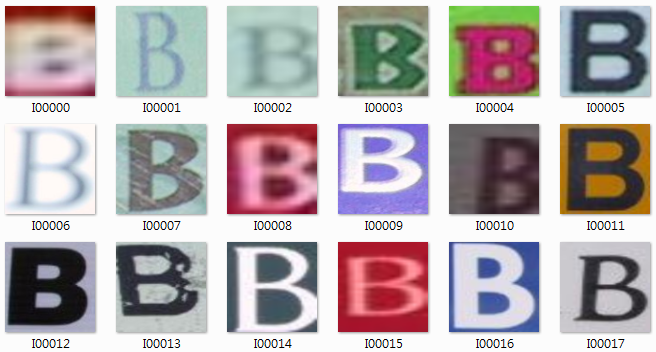
\includegraphics[width=1\linewidth]{fig/train_data}
\end{center}
   \caption{Examples of truncated training data. Notice that the internal geometric information still preserved after eliminate information on both sides.}
\label{fig:sample1}
\end{figure}

\begin{figure*}[ht]
\begin{center}$
\begin{array}{cc}
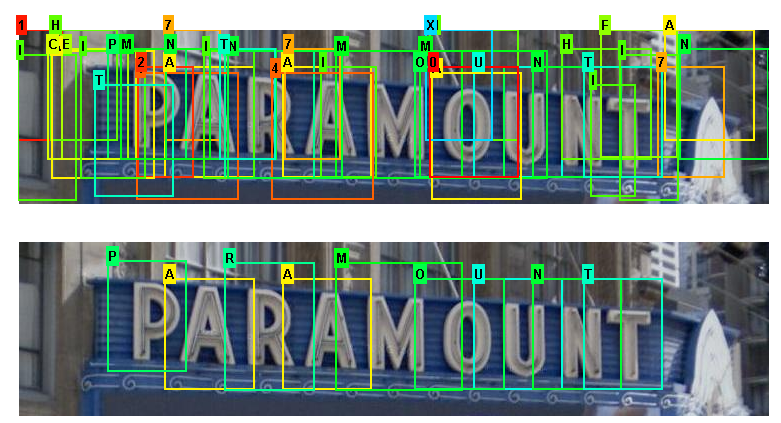
\includegraphics[width=1\linewidth]{fig/p13_after}
\end{array}$
\end{center}
\caption{Illustration of character detection and word recognition.}
\label{figure:end-to-end}
\end{figure*}

%-------------------------------------------------------------------------
\section{Word Recognition}

The character detection step provides us with a large amount of potential candidate bounding boxes for each character. Our next step is to find words from those candidates and produce reliable word recognition output.

\subsection{Problem setup}

Let $x=(x_{1},...,x_{n})$ be the candidates bounding boxes and $s=(s_{1},...,s_{n})$
be the scores associated with them. We want to find the optimal configuration
that minimizes the following cost function
\begin{eqnarray*}
x^{*} & = & argmin-s^{T}x+x^{T}Ax\\
s.t &  & x_{i}(x_{i}-1)=0\forall i=1...n
\end{eqnarray*}
where A is a cost matrix. The construction of the Given the primal problem, the dual of this problem is derived as followed,
\begin{eqnarray*}
d^{*} & = & max-\frac{1}{2}(s+\lambda)^{T}(A+\mbox{diag}(\lambda))^{\dagger}(s+\lambda)\\
s.t. &  & A+\mbox{diag}(\lambda)\succeq0\\
 &  & s+\lambda\in\Re(A+\mbox{diag(\ensuremath{\lambda}))}
\end{eqnarray*}
The semidefinite programming equivalent of this problem is expressed as followed,

\begin{eqnarray*}
\max t\\
s.t &  & \left[\begin{array}{cc}
A+\mbox{diag}(\lambda) & -\frac{1}{4}(s+\lambda)\\
-\frac{1}{4}(s+\lambda) & -t
\end{array}\right]\succeq0
\end{eqnarray*}
The dual of the SDP is

\begin{eqnarray*}
d^{*} & = & \mbox{argmin} tr(AZ)-\frac{1}{2}s^{T}z\\
s.t. &  & diag(Z)=\frac{1}{2}z\\
 &  & \left[\begin{array}{cc}
Z & z\\
z^{T} & 1
\end{array}\right]\succeq0
\end{eqnarray*}
We treat this SDP problem as a relaxation of the primal problem. After obtaining the solution for the SDP, we search across the values of z as thesholds to minimize the original cost function.
\subsection{Constructing}
\subsection{Word Re-scoring and NMS}

The final step is our algorithm is to perform word level re-scoring and NMS~\cite{417} in order to capture global information for each word output by pictorial structure.

%-------------------------------------------------------------------------
\section{Experiment}

This section describes detailed evaluation of our method.

\subsection{Dataset}

We use the Street View Text (SVT)~\cite{417} dataset in our experiments. The SVT dataset contains images taken from Google Map Street View. The words in SVT images come from local business sign and have high degree of variability in appearance and resolution. There are total $647$ cropped word images from the SVT testing set.

\subsection{Character Detection}

There are many descriptors can be used for character recognition, and we choose the HOG feature as our descriptor that it outperform the others in~\cite{117} because it preserves better geometric information. We densely compute HOG features with a cell size of $8 \times 8$ using $8$ bins after resizing each image to $48 \times 48$ windows. This character detector is trained on ICDAR 2003 dataset, char74K, and our synthetic data using a one-againt-one SVM classifier with an RBF kernel, where the synthetic data contains about 10,000 images for 62 classes using 40 fonts and for each image we add some amount of Gaussian noise, and apply a random affine deformation.

We then perform sliding window based character detection for multi-scale and multi-aspect ratio for every location in the input image. The candidate bounding boxes obtained by SVM classifier are then pruned by normal distribution model with a probability less than $0.4$. NMS is performed on the remaining bounding boxes to avoid wrong elimination. These two pruning steps are simply but efficient to discard noisy candidate while still preserve most true positive candidates for the next word recognition step.

\subsection{Cropped Word Recognition}

We evaluate cropped word recognition on the SVT-WD dataset assuming a perfect text detector is available. Pictorial structure in~\cite{417} is used to recognize words using a lexicon of about $50$ words for each image. Figure ~\ref{figure:result1} shows the output by our system compared with the previous work in ~\cite{417}. Table ~\ref{table:compare} shows the word recognition accuracy is improved using multi-scale and multi-aspect ratio approach, and the result could be further improved by training on truncated training (TT) data total $10\%$ more.

\begin{table}
\begin{center}
\begin{tabular}{|l|c|}
\hline
Approach & Accuracy \\
\hline\hline
Previous work~\cite{417}  & 0.56 (364 words) \\
Multi-scale + Multi-ratio & 0.60 (390 words)\\
Multi-scale + Multi-ratio + TT & 0.66 (427 words)\\
\hline
\end{tabular}
\end{center}
\caption{Cropped Word Recognition Accuracy: A comparison of proposed method to PLEX in~\cite{417}. We improve the accuracy by $10\%$ in SVT-WORD dataset.}
\label{table:compare}
\end{table}

\subsection{Results and Discussion}

We evaluate our methods on the challenging SVT dataset, which contains words in different viewpoints, sizes/scale, locations, fronts, and styles with low resolution or low contract conditions. We observe that our proposed method outperform~\cite{117} in cropped word recognition by $10\%$.

We study the effect of multi-ratio of width and height. Original work in~\cite{417} uses fixed aspect ratio for sliding window approach. However, we observe that different characters tend to have different ratios between width and height. In order to leverage this feature, multi-ratio of width and height for sliding window is performed in our algorithm, and the word recognition accuracy is higher by $4\%$ as in Table~\ref{table:compare}. The reason could be that our multi-ratio approach can better capture true character bounding boxes in natural image with high variability.

We also analyze the effect of truncated training data. Random Fern classifier is train on square training data that contain some noise on both sides in~\cite{417} .However, in many real street view cases, characters are tightly connected and it is difficult to contain all possible noise in training step. Therefore, we train our character detector on truncated training data by discarding $0.3$ width information on both sides to capture the internal geometric information. The training error is higher than before by using truncated training data but surprisingly the word recognition accuracy is higher by $6\%$ more and achieve total $10\%$ higher (Table~\ref{table:compare}) in cropped word recognition accuracy than in~\cite{417}. The result shows that we only need the internal information to capture characters in natural street view image and we can avoid the labor of collecting all possible combinations for the noise in both sides in training step. In the reminder of the paper we will refer to the truncated training procedure as ``TT''

\begin{figure}
\begin{center}$
\begin{array}{cc}
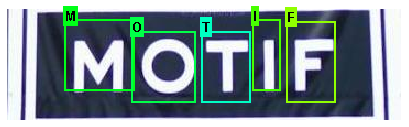
\includegraphics[width=1\linewidth]{fig/p9} \\
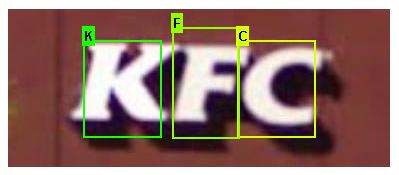
\includegraphics[width=1\linewidth]{fig/p11} \\
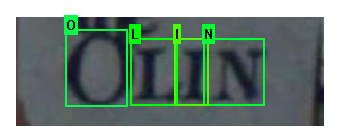
\includegraphics[width=1\linewidth]{fig/p12} \\
\end{array}$
\end{center}
\caption{Experiment results on SVT-WORD dataset.}
\label{figure:result1}
\end{figure}

%-------------------------------------------------------------------------
\section{Conclusion}

Our work establish a new approach to improve traditional sliding window based character detector and a novel way to select useful training data by truncating each character on both sides and further extract more representative geometric information for character classifier. We show that we can outperform original work in~\cite{417} for both cropped word recognition and ene-to-end scene text recognition on full images, and contribute to better text recognition in the natural images.


{\small
\bibliographystyle{ieee}
\bibliography{egbib}
}

\end{document}
